%追加すべき事項
% - 各種アルゴリズムの説明
% - 実験結果の画像の添付
\appendix
\chapter{学習時のパラメータ}
\label{sec:appendix_params}

提案モデルの学習時のパラメータの値を表\ref{tab:params1}に示す。また、Adam~\cite{Adam}の疑似コード~(Algorithm~\ref{alg:Adam})~にあるハイパーパラメータの値を表\ref{tab:params2}に示す。

\begin{table}[b]
\begin{center}
\begin{minipage}{0.49\hsize}
    \begin{center}
        \begin{tabular}{lr}\toprule
            パラメータ & 値 \\ \midrule
            バッチサイズ & 1 \\ 
            エポック数 & 1000 \\ \bottomrule
        \end{tabular}
    \end{center}
    \caption{}
    \label{tab:params1}
\end{minipage}
\begin{minipage}{0.49\hsize}
    \begin{center}
        \begin{tabular}{lr}\toprule
            パラメータ & 値 \\ \midrule
            $\beta_1$ & 0.5 \\
            $\beta_2$ & 0.999 \\
            $\eta$ & 0.0002 \\ 
            $\epsilon$ & $10^{-8}$ \\ \bottomrule
        \end{tabular}
    \end{center}
    \caption{}
    \label{tab:params2}
\end{minipage}
\end{center}
\end{table}

\begin{algorithm}[b]
\label{alg:Adam}
    \DontPrintSemicolon
    %\SetAlgoNoEnd\SetAlgoNoLine
    \SetKwInOut{KwHyParam}{HyperParameter}
    \SetKwInOut{KwParam}{Parameter}
    \SetKwInOut{KwObFunc}{Objective~Function}
    \KwHyParam{$\beta_1,\beta_2\in \interval[open left]{0}{1},\eta,\epsilon$}
    \KwObFunc{$f$}
    \KwParam{$\theta$}
    \Init{
        \settowidth{\maxwidth}{$m_1,m_2 \leftarrow 0,0$~}
        \algalign{$t \leftarrow 0$~}{(Initialize~timestep)\;}
        \algalign{$\theta \leftarrow \theta_0$~}{(Initialize~Parameter)\;}
        \algalign{$m_1,m_2 \leftarrow 0,0$~}{(Initialize~moments)\;}
    }
    \Proc{
        \While{$\theta$ not converged}{
            \settowidth{\maxwidth}{$m_1,m_2 \leftarrow \beta_1 \cdot m_1+(1-\beta_1) \cdot g,\beta_2 \cdot m_2+(1-\beta_2) \cdot (g \odot g)$~}
            \algalign{$t \leftarrow t+1$~}{(Update~timestep)\;}
            \algalign{$g \leftarrow \nabla _{\theta} f(\theta)$~}{(Compute~gradient~of~$f(\theta)$)\;}
            \algalign{$m_1,m_2 \leftarrow \beta_1 \cdot m_1+(1-\beta_1) \cdot g,\beta_2 \cdot m_2+(1-\beta_2) \cdot (g \odot g)$~}{(Update~biased~moments)\;}
            \algalign{$\hat{m_1},\hat{m_2} \leftarrow m_1/(1-\beta_1^t),m_2/(1-\beta_2^t)$~}{(Update~bias-corrected~moments)\;}
            \algalign{$\theta \leftarrow \theta - \eta \cdot \hat{m_1}/(\sqrt{\hat{m_2}}+\epsilon)$~}{(Update~Parameter)\;}
        }
        \Return{$\theta$}\;
    }
\caption{Adam~\cite{Adam}の疑似コード}
\end{algorithm}

\chapter{データセットの分割}
\label{sec:appendix_split}

22音ずつの4つのサブセットにデータセットを分割した~(図\ref{fig:data_div})~。また、データセットの4分割は、88音をシャッフルして配列に格納した後に22音ずつ順に選ぶことで実装した。

\begin{figure}[h]
\begin{center}
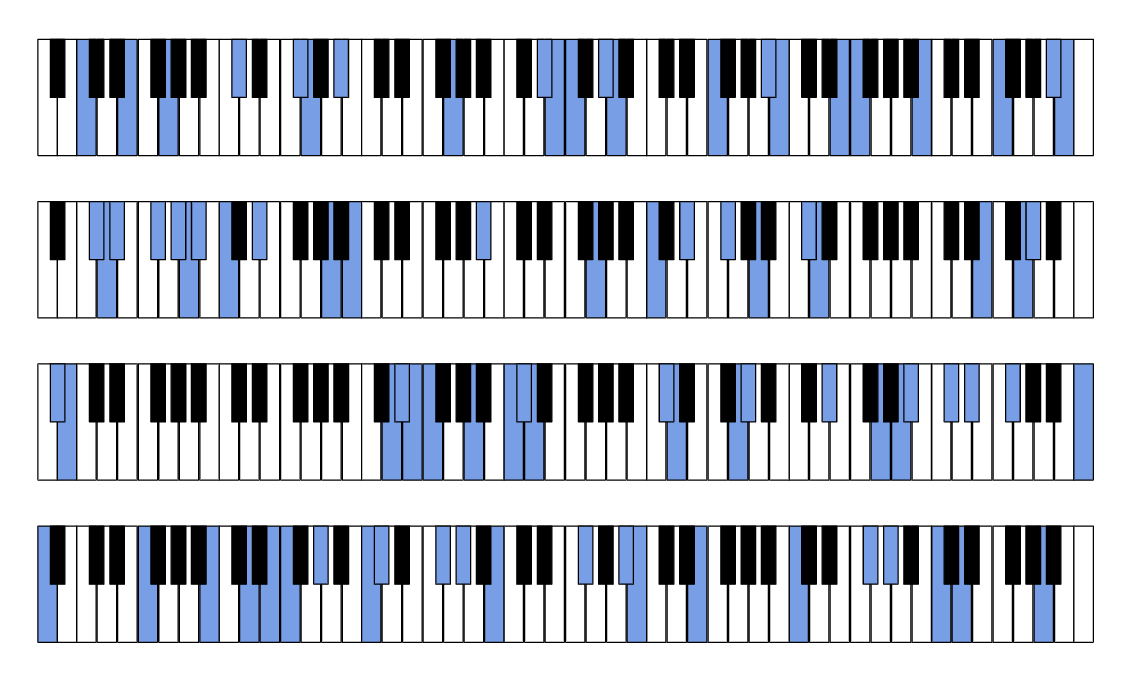
\includegraphics[width=\hsize]{figure/data_div.png}
\caption{データセットのサブセット}
\label{fig:data_div}
\end{center}
\end{figure}

\chapter{実験結果}
\label{sec:appendix_result}

\ref{result}節に載せることのできなかった波形の図を本章に載せる

\section{提案モデルの表現力の評価実験}

提案モデルの評価実験を行ったところ、88音のうち87音については変換先のギターの音を表現できていると判断することができた。


\section{提案モデルの汎化能力の評価実験}